\chapter{Benchmark und Modellauswahl}\label{ch:benchmark}

Die systematische Auswahl eines geeigneten \glspl{llm} erforderte die Entwicklung und Anwendung eines spezifisch auf den Anwendungsfall zugeschnittenen Benchmarks.
Die Konzeption und Durchführung war ein iterativer Prozess bei dem stetig Erkenntnisse und identifizierte Probleme dazu genutzt wurden, die Rahmenbedingungen des Benchmarks zu verbessern.
Dieser iterative Prozess hatte zur Folge, dass aufbauend auf Zwischenergebnisse Anpassungen vorgenommen wurden.
Deshalb wird in den folgenden Unterkapiteln nicht nur auf das finale Ergebnis des Benchmarks, sondern auch auf die Zwischenergebnisse und die daraus abgeleiteten Entscheidungen eingegangen.

% ======================================================================================================================

\section{Auswahl der Sprachmodelle}\label{sec:modelle-benchmark}

Die Auswahl an verfügbaren \glspl{llm} wird einerseits durch die Leistungsfähigkeit der verwendeten Hardware und andererseits durch die Kompatibilität der Software eingeschränkt.
Erste Experimente ergaben, dass der verwendete Mac Mini M4 Pro mit 64 Gigabyte Arbeitsspeicher \glspl{llm} mit einer Parametergröße von maximal 108 Milliarden ausführen kann, ohne wärmebedingt die Leistung zu drosseln.
Da die finale Implementierung des Benchmarks softwareseitig mit Ollama4J einen lokal ausgeführten Ollama Server anspricht, konnten nur solche \glspl{llm} ausgewählt werden, die auf Ollama zur Verfügung stehen.
Die Wahl an \glspl{llm}, die für den Benchmark genutzt werden sollen, beschränkt sich somit auf Modelle die durch Ollama unterstützt werden und bis zu 108 Milliarden Parameter groß sind.
Es wurden \glspl{llm} von zahlreichen namhaften Providern geprüft, darunter Microsoft (phi4, phi3), Meta (llama4, llama3), Deepseek (deepseek-coder, deepseek-r1), Alibaba (qwen3, qwen2.5, qwen2.5-coder), Google (gemma3, gemma3n) und Mistral (mistral, mathstral, devstral, mistral-small, mistral-nemo).
Zusätzlich zu etablierten Modellen wurden auch gezielt exotischere und weniger verbreitete Modelle ausgewählt (llava, olmo2, orca-mini, dolphin).
Neben den Providern spielte auch die ausgeschriebene Verwendung der Modelle eine Rolle, somit wurden Modelle für verschiedene Anforderungen wie Vision (llava), Reasoning (qwen3, mixstral) und Programmierung (devstral, qwen2.5-coder) ausgewählt.
Um einen Vergleich in Hinsicht auf Präzision und Performance anhand der Modellgröße zu ermöglichen, wurden gezielt kleine Modelle (tinyllama:1.1b, orca-mini:3b, qwen2.5-coder:0.5b), mittelgroße Modelle (mistral-small:24b, qwen2.5-coder:32b) und große Modelle (llama4:108.6B, mixstral:8x7b) verglichen.
Die finale Durchführung des Benchmarks umfasste 30 \glspl{llm}.

% ======================================================================================================================

\section{Konzeption}\label{sec:konzeption-benchmark}

Ziel des Benchmarks ist es, ein geeignetes \gls{llm} zu bestimmen.
Es wird geprüft, inwiefern jedes \gls{llm} Copyright-Informationen extrahieren kann, die Policy-konformen Erwartungshaltungen entsprechen.
Hierzu wird das \gls{llm} mit einem Prompt dazu aufgefordert, die Copyright-Statements, Urheber und Autoren für eine bestimmte Eingangsdatei zu bestimmen und anschließend wird die Antwort des \gls{llm} mit einer vorher formulierten Erwartungshaltung abgeglichen.
Dieser Schritt wird für jede Datei des Benchmark-Datensatzes durchgeführt.
Der verwendete Datensatz wird im Abschnitt \nameref{sec:datensatz-benchmark} thematisiert.
Anschließend werden die Ergebnisse des \gls{llm} anhand mehrerer Metriken ausgewertet und mit den Ergebnissen anderer \glspl{llm} verglichen.

\begin{figure}[ht]
    \centering
    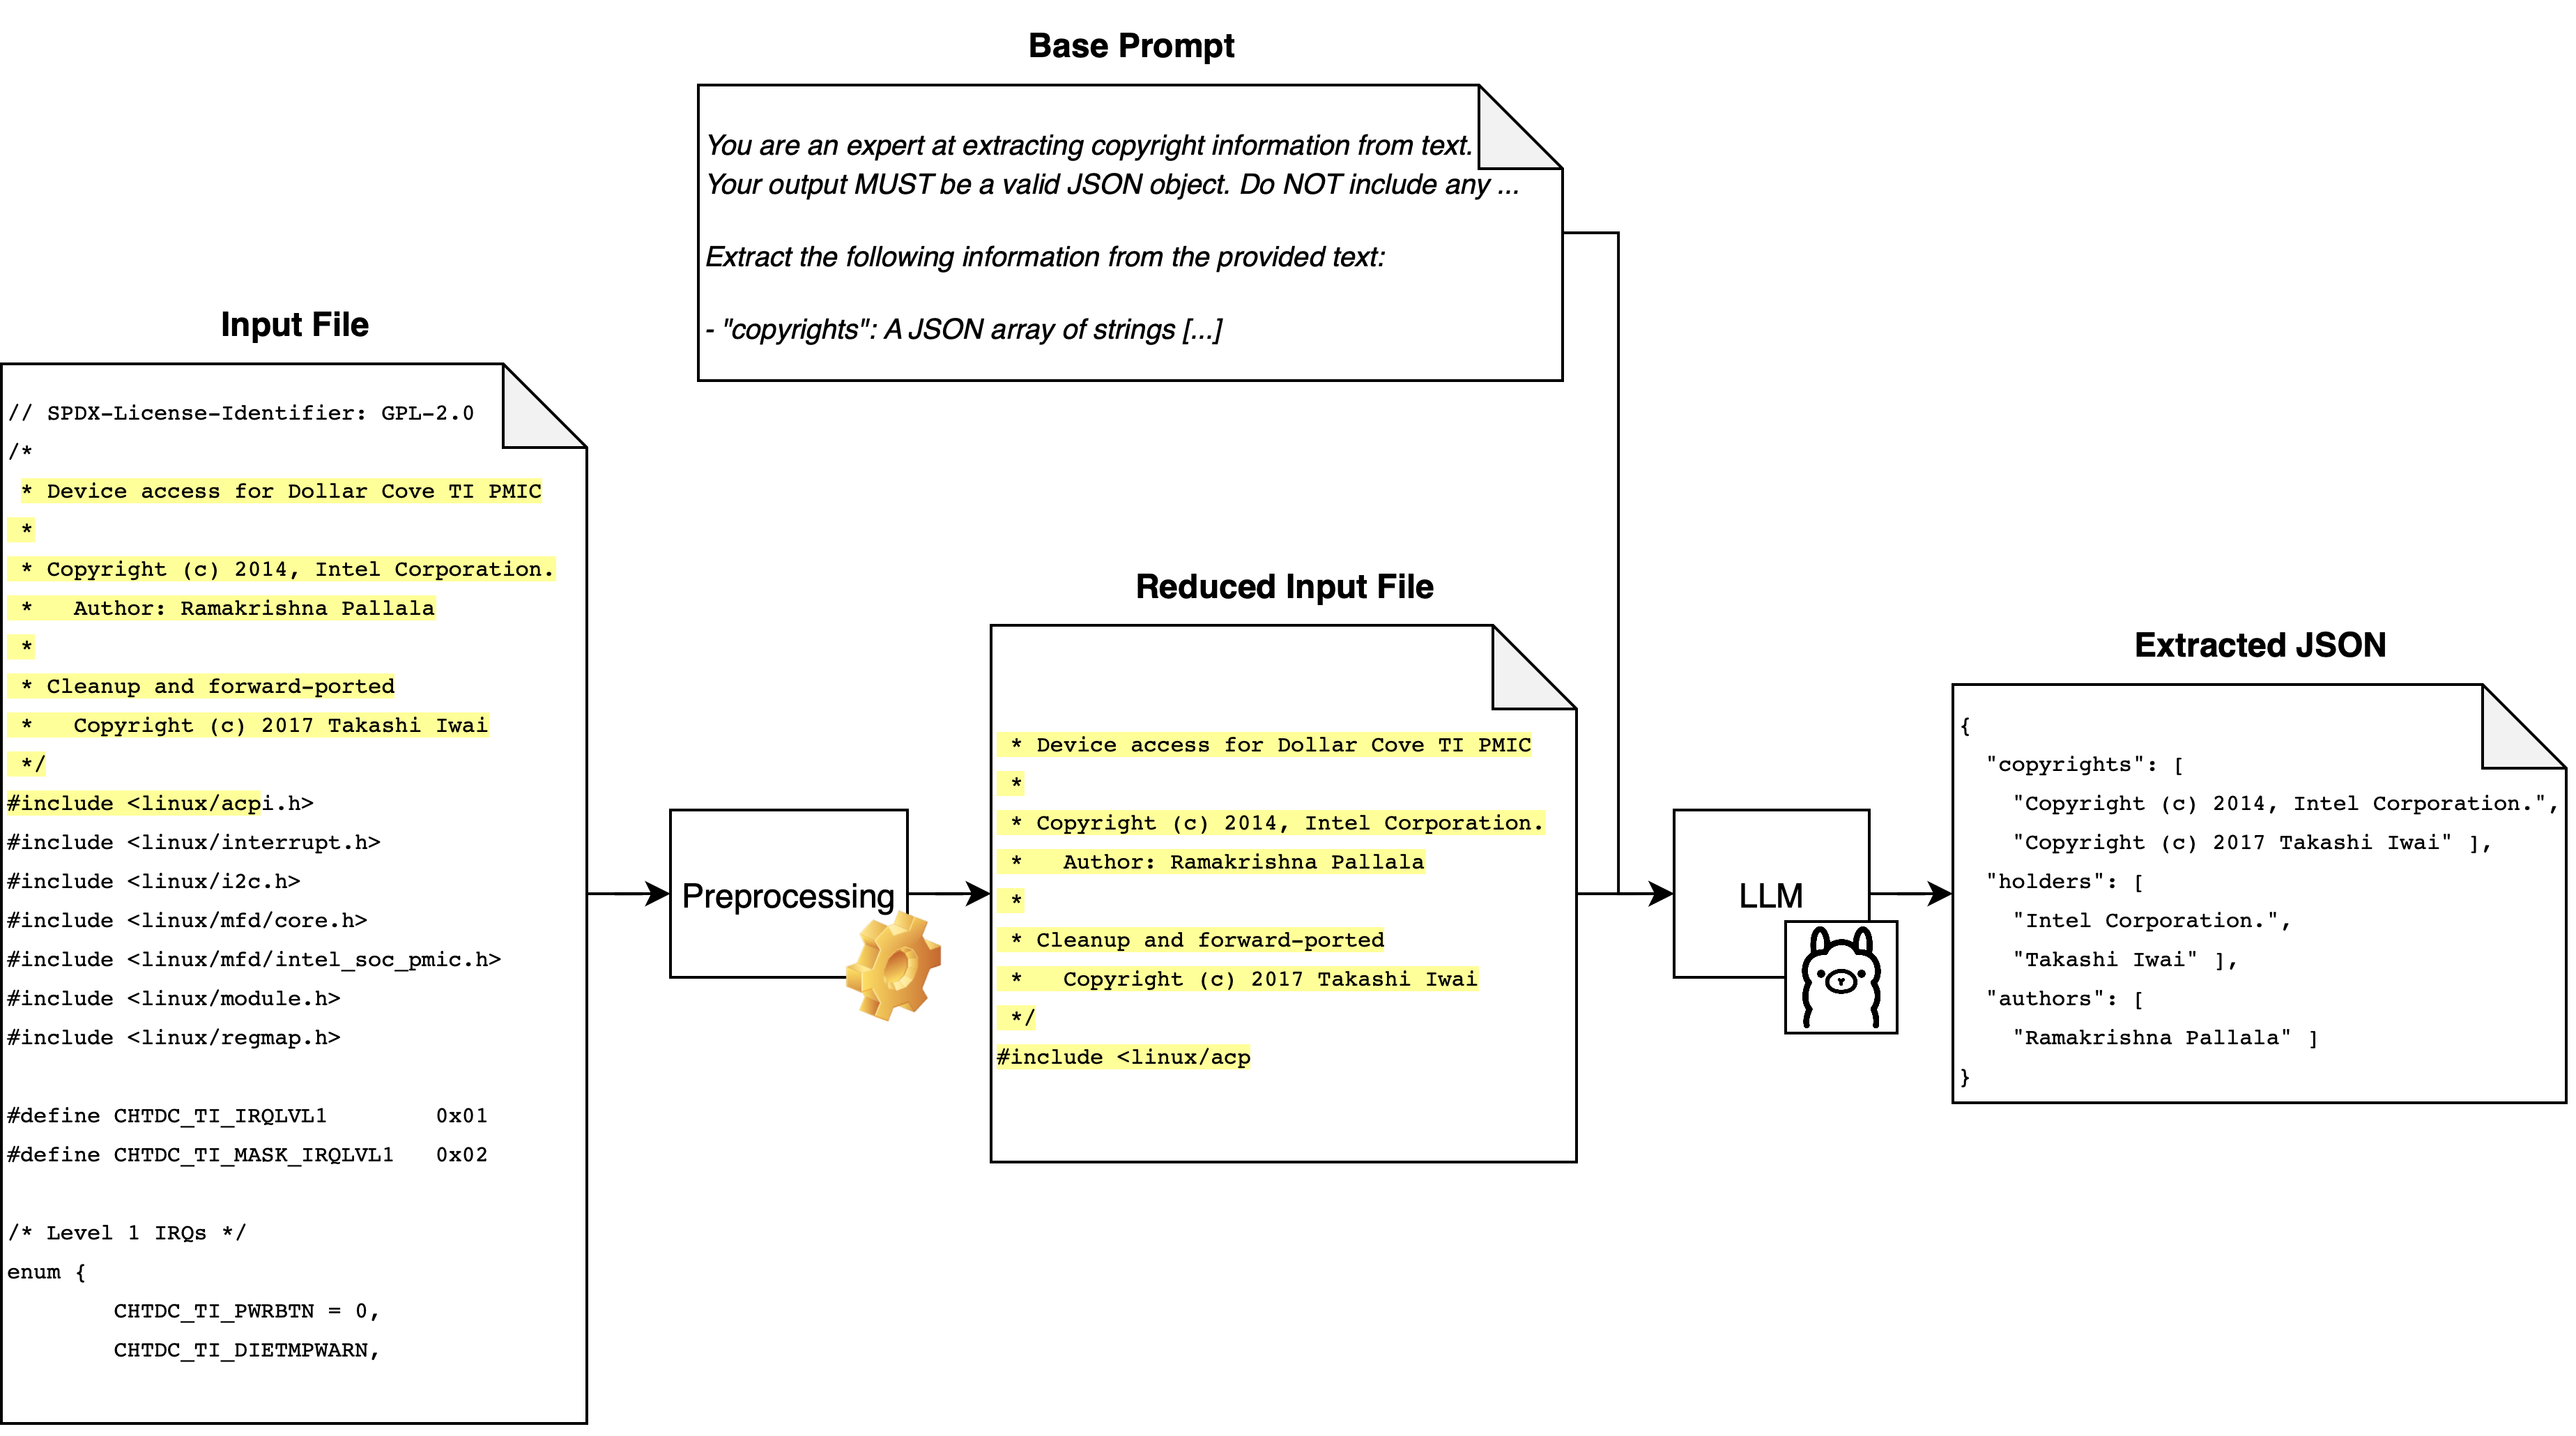
\includegraphics[width=15cm]{benchmark/prompting}
    \caption{Ablauf des Benchmarks}
    \label{fig:prompting_setup}
\end{figure}

% ----------------------------------------------------------------------------------------------------------------------

\subsection{Lokale Ausführung der LLMs}\label{subsec:lokale-ausfuehrung}

Um konsistente Ergebnisse über mehrere Durchläufe hinweg zu erzielen, muss sichergestellt werden, dass die Ausgaben der Modelle für denselben Prompt bei mehrmaliger Durchführung nicht variieren.
Hierzu wird die Temperatur der \glspl{llm} auf 0,0 gestellt.
Diese Einstellung ermöglicht es, die Varianz zwischen den Ausgaben, welche bei kreativer Textgenerierung durchaus erwünscht ist, zu eliminieren und sorgt somit für eine deterministische Ausgabe.
Die Funktionalität der Temperatur wurde praktisch geprüft, indem ein Modell in einer bestimmten Größe und Version auf zwei verschiedenen Endgeräten mit demselben Prompt angewiesen wurde und in beiden Fällen eine identische Ausgabe generierte.
Um sicherzustellen, dass im Verlauf des Benchmarks und darüber hinaus keine Updates der Modelle die Ergebnisse verfälschen, müssen feste Versionen der \glspl{llm} verwendet werden.
Da proprietäre \glspl{llm} wie ChatGPT oder Gemini keine Steuerung der Versionen oder Temperatur ermöglichen, ist eine lokale Ausführung der Modelle erforderlich.
Außerdem fallen für die Nutzung der \gls{api} dieser Modelle kosten an, weshalb eine lokale Ausführung auch hier zu bevorzugen ist.
Allerdings erfordert die lokale Ausführung der Modelle, dass diese auf der vorhandenen Hardware lauffähig sind, dies beschränkt die Auswahl der Modelle auf kleinere Parametergrößen und durch \gls{glos:quantisierung} verkleinerte Modelle.

% ======================================================================================================================

\section{Implementierung}\label{sec:benchmark-implementierung}

Für die Umsetzung des Benchmarks wurde ein Java-basiertes Backend entwickelt, das über die Bibliothek Ollama4J\footnote{\url{https://github.com/ollama4j/ollama4j}} mit einem lokal ausgeführten\gls{llm} kommuniziert.
Ollama4J stellt Java-Bindings für Ollama\footnote{\url{https://ollama.com}} bereit, eine leichtgewichtige Laufzeitumgebung für \glspl{llm}, die über eine standardisierte REST-API angesteuert wird.
Die Verwendung von Ollama ermöglichte eine einfache Modellanbindung sowie ein benutzerfreundliches Modellmanagement.
Eine Alternative zu Ollama stellt llama.cpp\footnote{\url{https://github.com/ggml-org/llama.cpp}} dar.

% Ollama vs llama.cpp
% Ollama4J verwendet
% Nutzung von TextSieve
% Model Warmup
% Erfassung aller Metriken pro Kategorie/File/Insgesamt
% Timeout von 5 Minuten mit Single-Thread Executor Service
% Parsing von JSON durch ChatUtil

% ======================================================================================================================

\section{Zusammenstellung des Datensatzes}\label{sec:datensatz-benchmark}

Die Ergebnisse der Datenaggregation wurden dazu genutzt, einen kuratierten Benchmark-Datensatz zu erstellen.
Hierzu wurden repräsentative Fälle aus der Datenaggregation identifiziert und ihre Erwartungshaltung anhand der Policy überprüft und wenn nötig, angepasst.
Der Datensatz umfasst insgesamt $n=200$ Dateien und ihre überprüften Erwartungshaltungen.
Die \num{200} Dateien sind in acht Kategorien mit jeweils \num{25} Dateien unterteilt:

\begin{itemize}
    \item single copyrights with authors
    \item single copyrights without authors
    \item multiple copyrights with authors
    \item multiple copyrights without authors
    \item case-insensitive matches
    \item format-insensitive matches
    \item only authors
    \item no copyrights or authors or holders
\end{itemize}

Die ersten vier Kategorien stellen die \enquote{normalen} Fälle dar, wobei die \textit{case-insensitive} und \textit{format-insensitive} Fälle speziell die Normalisierungen des ScanCode-Toolkits abdecken.
Die Kategorien \textit{no copyrights or authors or holders} und \textit{only authors} dienen gezielt dazu, das Verhalten des Modells bei Abwesenheit von Copyright-Statements zu untersuchen sowie die alleinige Autorenextraktion.
Um repräsentative Fälle einer Kategorie zusammenzustellen wurden je \num{25} Dateien aus den Hauptkategorien des Datensatzes zufällig ausgewählt und anschließend gesichtet.
Ähnliche Fälle (z.B.\ mehrere Copyright-Statements desselben Urhebers) wurden identifiziert und entsprechend ersetzt.
Somit konnte sichergestellt werden, dass kein Copyright, Urheber oder Autor überrepräsentiert im Datensatz vorkommt.
Die relativ kleine Anzahl von Dateien wurde dadurch kompensiert, dass mithilfe der Kategorien möglichst unterschiedliche Arten von Statements und Autoren im Benchmark enthalten sind.
Darüber hinaus ist jede Kategorie mit derselben Anzahl an Dateien vertreten, wodurch eine Bevorzugung bzw.\ Benachteiligung eines Modells anhand ungleichmäßiger Verteilung von Fällen zusätzlich mitigiert wird.
Die Formulierung der Erwartungshaltungen der ausgewählten Dateien wurde anhand einer reduzierten Policy durchgeführt.
Die reduzierte Policy enthielt lediglich die \nameref{subsec:cir-01}, sowie die \nameref{subsec:cep-01} und \nameref{subsec:cep-02}, wobei die \nameref{subsec:hir-01} und \nameref{subsec:air-01} implizit umgesetzt wurden, da sie zu diesem Zeitpunkt noch nicht ausreichend formuliert waren.

% ======================================================================================================================

\section{Metriken}\label{sec:metriken-benchmark}

Eine systematische Analyse der Eignung mehrerer \glspl{llm} erfordert mehrere Metriken die zur Evaluation herangezogen werden.
Die in diesem Benchmark verwendeten Metriken werden nachfolgend erläutert dabei werden die generierten Ergebnisse des \gls{llm} wie folgt interpretiert:
\begin{itemize}
    \item \textit{\gls{tp}} -- ein Element aus der Erwartungshaltung wird korrekt extrahiert (entweder exakte oder ausreichend ähnliche Übereinstimmung). Sofern ein \gls{tp} für ein Element aus der Erwartungshaltung gefunden wurde, wird dieses Element für die weitere Bewertung ausgeschlossen da jedes Element nur einmalig zugewiesen werden kann.
    \item \textit{\gls{fp}} -- ein vom Modell extrahiertes Element ist nicht in der Erwartungshaltung enthalten oder es ist verbleibt kein ausreichend ähnliches Element.
    \item \textit{\gls{fn}} -- ein Element aus der Erwartungshaltung wird vom Modell nicht extrahiert (weder exakte noch ausreichend ähnliche Übereinstimmung).
\end{itemize}

\subsection{Exact Matches}
Die zentrale Metrik zur Bewertung der Extraktion von Copyright-Statements ist der Anteil sogenannter \textit{Exact Matches}.
Ein \textit{Exact Match} liegt vor, wenn ein vom \gls{llm} generiertes Statement exakt mit einem Statement der vorher formulierten Erwartungshaltung übereinstimmt.
Durch eine perfekte Extraktion ohne zusätzliche Zeichen oder fehlerhafte Normalisierungen wird die \nameref{subsec:cep-01} erfüllt.
Mehrere Studien nutzen \textit{Exact Matches} als Bewertungsmaß für die Leistung von \gls{ner}- und \gls{ie}-Systemen auf Basis von \glspl{llm} \autocite{dunn_structured_2022}\autocite{hu_improving_2024}.

\subsection{F1-Score}
Eine gängige Metrik zur Bewertung von Klassifikationsmodellen ist der F1-Score\autocite{noauthor_f-score_2025}.
Der F1-Score stellt das harmonische Mittel aus Präzision (\textit{P}) und Recall (\textit{R}) dar.
Die Formeln für \textit{P}, \textit{R}, und \textit{F1} lauten wie folgt:

\[
 P = \frac{\mathrm{TP}}{\mathrm{TP} + \mathrm{FP}}
\]

\[
 R = \frac{\mathrm{TP}}{\mathrm{TP} + \mathrm{FN}}
\]

\[
 F1 = 2 \times \frac{P \times R}{P + R}
\]

Außerdem wird ein kombinierter F1-Score aller Elemente einer Eingabe $\mathrm{F1}_{overall}$ berechnet:

\[
 \mathrm{F1}_{overall} = \frac{\mathrm{F1}_{copyrights} + \mathrm{F1}_{holders} + \mathrm{F1}_{authors}}{3}
\]

In diesem Benchmark wird für jeden Entitätstyp der jeweilige F1-Score berechnet und zusätzlich ein durchschnittlicher F1-Score über alle Typen hinweg erfasst.
Zunächst wird jedes extrahierte Copyright-Statement auf einen \textit{Exact Match} mit der Erwartungshaltung geprüft, liegt dieser vor, wird das Statement als \gls{tp} gezählt.
Sofern kein \textit{Exact Match} vorliegt, wird die Jaro-Winkler-Ähnlichkeit\autocite{noauthor_jarowinkler_nodate} verwendet um das ähnlichste Element aus der Erwartungshaltung welches einen Similarity-Threshold vom \num{0,95} überschreitet, zu finden.
Wenn eine solche Übereinstimmung gefunden wird, zählt diese als \gls{tp}.
Bei Holders und Authors wird ausschließlich durch die Jaro-Winkler-Ähnlichkeit auf ähnliche Elemente in der Erwartungshaltung geprüft und entsprechende Fälle werden als \gls{tp} gezählt.

\subsection{Tokens/sec}
Zur zeitlichen Messung der Modellleistungen werden die \textit{Tokens/sec} berechnet.
Da Ollama4J keine Abfrage der tatsächlichen Token pro Sekunde eines Modells unterstützt muss eine Alternative herangezogen werden.
Um die Leistung der unterschiedlichen Modelle zu bestimmen, wird berechnet wie groß der Eingabe-Prompt ist und wie viel Zeit das Modell zur Bearbeitung benötigt.
Die größe eines Prompts wird in Tokens gemessen, da die Modelle aber intern unterschiedliche Prozesse zur Tokenisierung eines Prompts verwenden, wird eine Annäherung verwendet.
Eine grobe Umrechnung von Eingabetext zu Tokens ist $1\;\text{Token}\approx 4\;\text{Buchstaben}$\autocite{noauthor_what_nodate}.
Die Dauer der Bearbeitung entspricht der Zeit zwischen dem Absenden des Eingabe-Prompts und der Beantwortung durch das Modell.
Die somit ermittelte Metrik stellt eine Vergleichbarkeit der Modell-Geschwindigkeit für alle \glspl{llm} dar, unabhängig von ihrer internen Tokenisierung.

% ======================================================================================================================

\section{Durchführung}\label{sec:durchfuhrung-benchmark}

% ----------------------------------------------------------------------------------------------------------------------

\subsection{Eingabeprompt}

% ======================================================================================================================

\section{Ergebnisse}\label{sec:ergebnisse-benchmark}

% ======================================================================================================================

\section{Wahl des Modells}\label{sec:auswahl-modell-benchmark}
